\chapter{Diffusion Models}\label{cap:15}

In questo capitolo affrontiamo una tematica profondamente diversa da quanto visto finora: l’utilizzo dei modelli di Deep Learning per la generazione di immagini. In precedenza, abbiamo esplorato l'approccio delle \textbf{Generative Adversarial Networks} (GAN), in cui si apprende direttamente la distribuzione di probabilità da cui si generano nuovi dati. Concentriamoci su una nuova metodologia: i \textbf{Modelli di Diffusione}, accanto a questi modelli, è importante segnalare l’emergere di una nuova famiglia di modelli generativi sviluppati nel 2024, i quali non verranno trattati in questi appunti. I modelli di diffusione si fondano su un'intuizione tanto semplice quanto potente: corrompere progressivamente un dato, aggiungendo rumore, fino a trasformarlo in rumore puro, per poi addestrare un modello per compiere il processo inverso, rimuovere gradualmente il rumore per recuperare l’immagine originale (Figura~\ref{fig:diffMod}). L’ispirazione teorica proviene dalla termodinamica, in cui i processi stocastici descrivono il passaggio da uno stato ordinato a uno disordinato e viceversa.
\begin{figure}[hbtp]
    \centering
    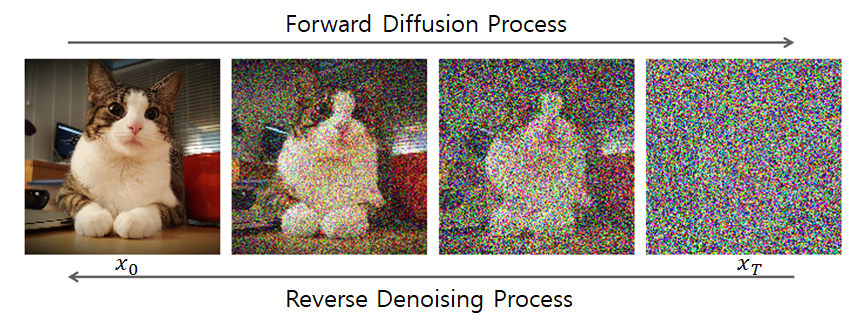
\includegraphics[width=\textwidth]{figure/diffusionModel}
    \caption{Schema di un modello di diffusione: nel processo forward si aggiunge rumore progressivamente a un’immagine, mentre nel processo inverso (Reverse Diffusion) si parte dal rumore per ricostruire l’immagine originale.}
    \label{fig:diffMod}
\end{figure}

\section{Stable Diffusion}
Una delle implementazioni più celebri ed efficienti di questa famiglia è \textbf{Stable Diffusion}. La sua innovazione principale consiste nel non applicare la diffusione direttamente sui pixel, ma su uno \textbf{spazio latente compresso}. Questo spazio, ottenuto tramite un Autoencoder, rappresenta le informazioni essenziali dell’immagine in una forma compatta e gestibile.

\begin{itemize}
    \item Il modello lavora con vettori di dimensioni molto più piccole rispetto ai pixel originali;
    \item Il costo computazionale e la memoria richiesta si riducono drasticamente;
    \item Il processo diventa più efficiente, pur mantenendo un'elevata qualità visiva.
\end{itemize}

Questa strategia ricorda quanto visto nei \textbf{Variational Autoencoder (VAE)}, dove si opera in uno spazio latente che cattura la struttura semantica dei dati.

\section{Task dei modelli di diffusione}

Stable Diffusion consente di affrontare diversi compiti di generazione, chiamati \textit{task}, tra cui:
\begin{itemize}
    \item \textbf{\texttt{text2img}:} generazione di immagini a partire da un prompt testuale;
    \item \textbf{\texttt{text+image}:} generazione o modifica di immagini a partire da un’immagine parziale e un prompt testuale.
\end{itemize}

In entrambi i casi, il modello è composto da tre moduli principali:
\begin{enumerate}
    \item \textbf{Text Encoder:} converte il testo del prompt in un embedding numerico (tramite il modello CLIP);;
    \item \textbf{Image Information Creator:} una rete U-Net che, insieme a uno scheduler, effettua il processo di denoising nello spazio latente;;
    \item \textbf{Image Decoder:} un Autoencoder che ricostruisce l’immagine finale dallo spazio latente.
\end{enumerate}

\begin{figure}[hbtp]
    \centering
    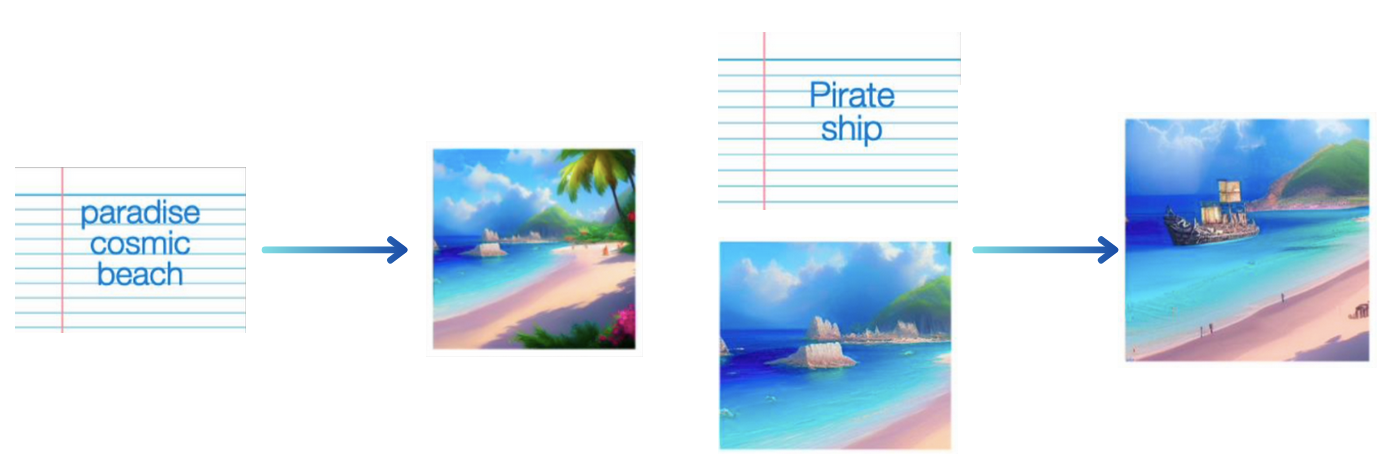
\includegraphics[width=0.7\textwidth]{figure/t2imgAndtextandtext}
    \caption{Esempio di task \texttt{text2img} (a sinistra), ed esempio di task \texttt{text+image} (a destra).}
    \label{fig:stabDiff}
\end{figure}

\section{Meccanismo di diffusione}
Il processo di diffusione si sviluppa in una serie di step progressivi. A ogni passo, il modello prende in input un vettore latente e lo aggiorna, aggiungendo o rimuovendo rumore a seconda della direzione del processo (forward o inversa). Durante la fase di generazione, il vettore latente viene gradualmente raffinato fino ad assumere la forma desiderata. Se osservassimo i risultati decodificati dopo ciascun passo, vedremmo immagini sempre più nitide, che da un semplice rumore convergono progressivamente verso un’immagine coerente con quanto richiesto (Figura~\ref{fig:stepDiff}).

\begin{figure}
    \centering
    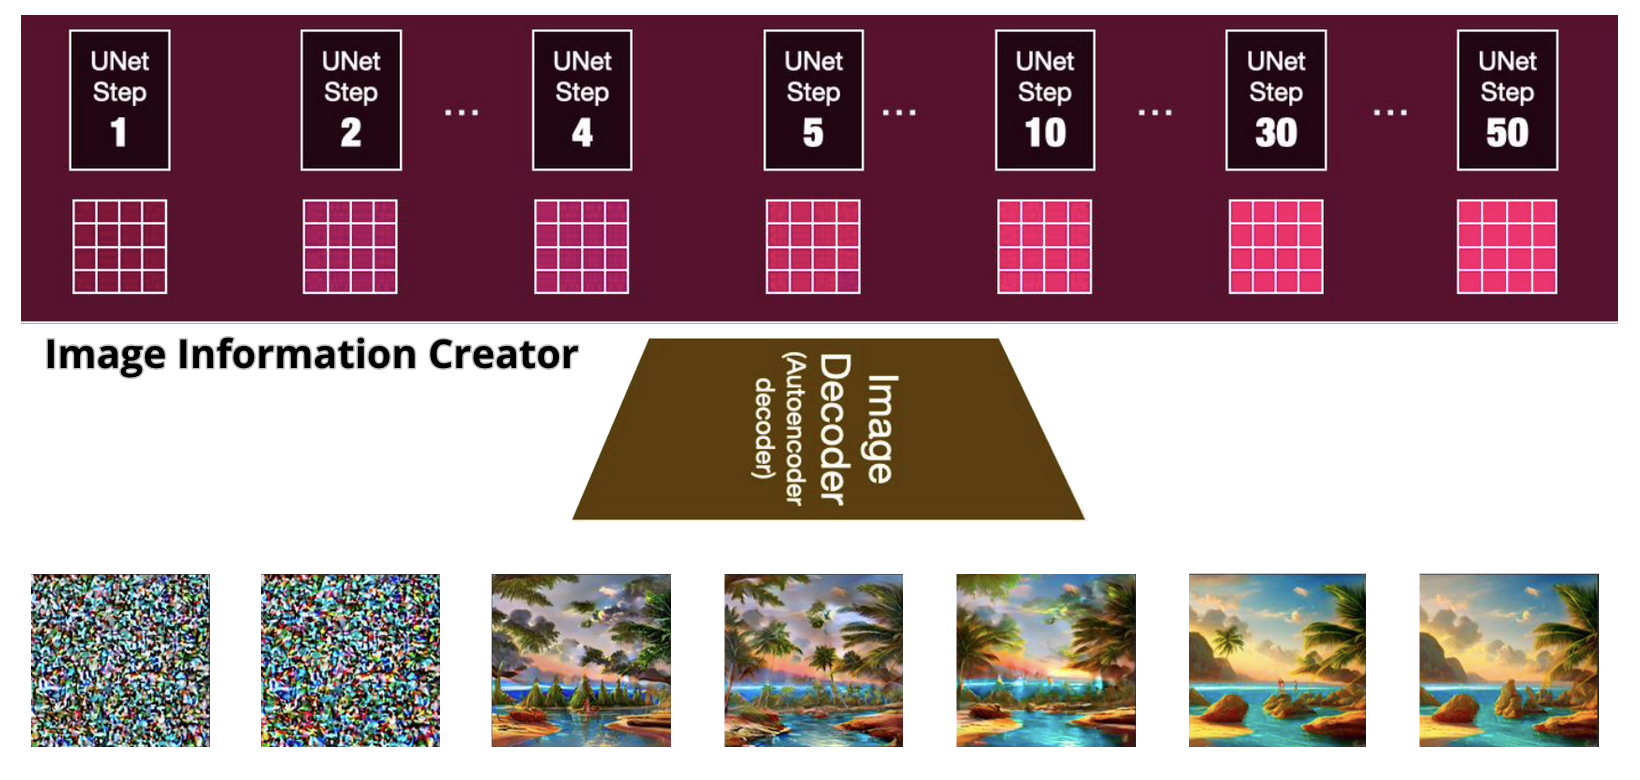
\includegraphics[width=\textwidth]{figure/DiffusionStep.png}
    \caption{Output decodificato progressivamente a ogni step della diffusione inversa.}
    \label{fig:stepDiff}
\end{figure}

\section{Diffusione inversa}

Il processo inverso è il cuore dei modelli di diffusione. Per ricostruire un’immagine dal rumore, il modello deve sapere quanto rumore è stato aggiunto a ogni passo. Per questo, si addestra una rete neurale, chiamata \textbf{Noise Predictor}, per stimare la quantità di rumore presente. L’addestramento segue questi passaggi:

\begin{enumerate}
    \item Si seleziona un'immagine dal dataset;
    \item Si genera una quantità casuale di rumore;
    \item Si corrompe l'immagine originale sommando il rumore;
    \item Si addestra la rete a predirre il rumore aggiunto.
\end{enumerate}
Durante la generazione (\textit{Denoising}), si parte da puro rumore e si sottrae, a ogni step, la stima del rumore fornita dal modello. Iterando il processo decine o centinaia di volte, il rumore scompare gradualmente, rivelando un’immagine coerente con quanto aspettato (Figura~\ref{fig:revDiff}).

\begin{figure}
    \centering
    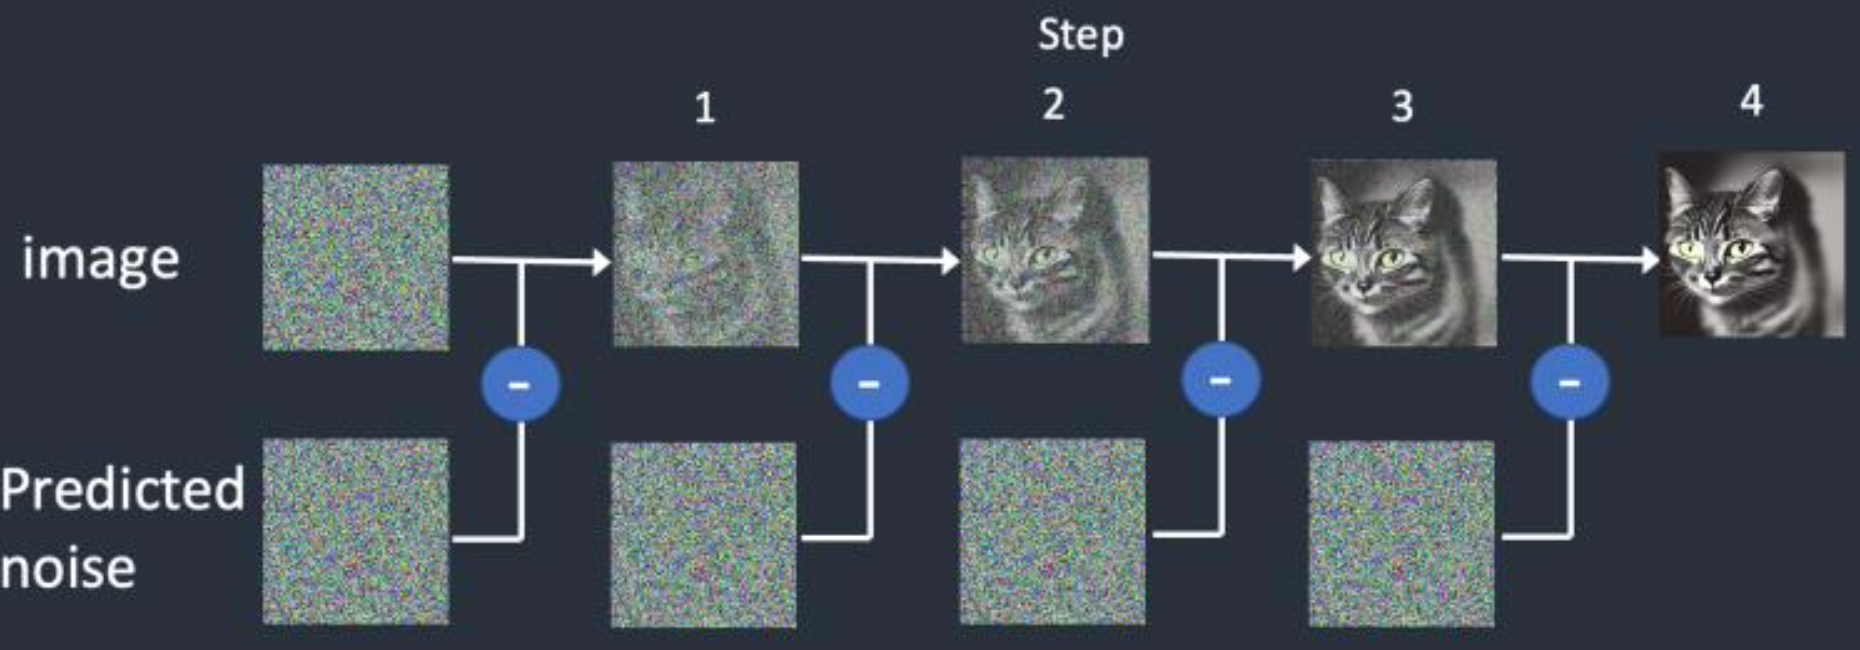
\includegraphics[width=\textwidth]{figure/ReverseDiffusion.png}
    \caption{Esempio di reverse diffusion: il rumore viene rimosso progressivamente fino a ottenere un’immagine pulita.}
    \label{fig:revDiff}
\end{figure}
Senza alcun vincolo esterno, questo processo è detto \textbf{incondizionato}, poiché il contenuto dell’immagine è determinato casualmente.

\section{Conditioning}

Per generare immagini coerenti con un prompt testuale, è necessario introdurre un meccanismo di \textbf{condizionamento} (\textit{conditioning}). In pratica, il modello non parte più solo dal rumore, ma riceve anche un’informazione aggiuntiva (il testo) che guida il processo di generazione. Il prompt viene elaborato da un \textbf{Text Encoder}, che produce un embedding vettoriale. Questo embedding viene poi integrato nella U-Net attraverso un meccanismo di \textbf{Cross-Attention}, consentendo al modello di generare contenuti visivi coerenti con la descrizione testuale.

\subsection{Cross-Attention}
Il meccanismo di \textbf{Cross-Attention} permette a una sequenza di essere "guidata" da un’altra. A differenza della \textit{Self-Attention}, dove una sequenza interagisce con sé stessa, qui l’interazione avviene tra due sequenze distinte (ad esempio, testo e immagine latente). Nel caso di Stable Diffusion:

\begin{itemize}
    \item Il \textbf{Text Encoder CLIP} genera un embedding per il prompt;
    \item La \textbf{U-Net} usa Self-Attention per la coerenza interna e Cross-Attention per collegarsi semanticamente al testo;
    \item Il risultato è un’immagine generata che riflette fedelmente il contenuto descritto nel prompt.
\end{itemize}

\subsubsection{CLIP}
Il modello \textbf{CLIP} (Contrastive Language–Image Pretraining) è fondamentale per collegare linguaggio e visione. Durante il suo addestramento, CLIP riceve coppie immagine-testo e impara a rappresentarle in uno spazio comune: due embedding (uno testuale e uno visivo) sono tanto più vicini quanto più l’immagine e la descrizione corrispondono semanticamente. Questa similarità viene misurata tramite la \textbf{cosine similarity} e ottimizzata via backpropagation.

\subsubsection{Cross-Attention nei Transformer}

Nel contesto dei Transformer, la Cross-Attention combina due sequenze: una da cui si ottengono le \textit{Key} e le \textit{Value}, e un’altra da cui derivano le \textit{Query}. L’output finale mantiene la dimensione della sequenza di Query.

\begin{figure}
    \centering
    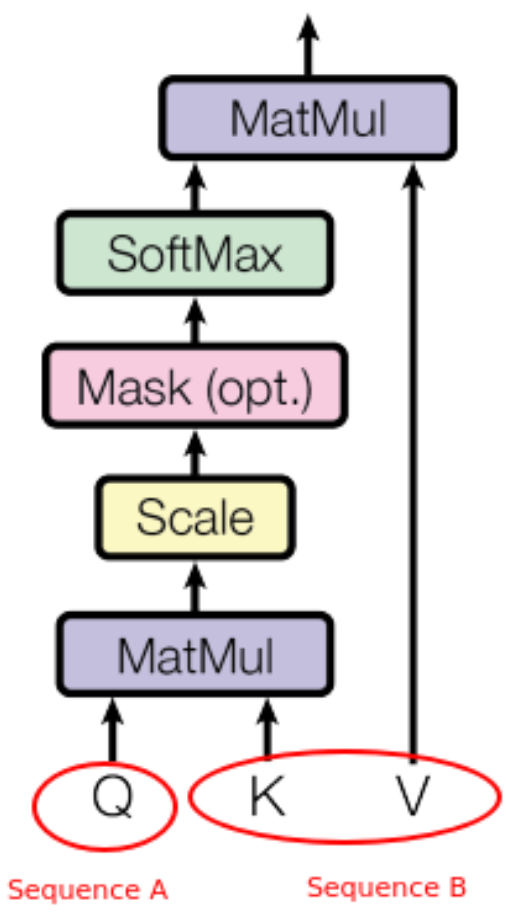
\includegraphics[width=0.2\textwidth]{figure/CrossTrasformer.png}
    \caption{Schema del meccanismo di cross-attention all'interno di un Transformer.}
    \label{fig:crossTrasf}
\end{figure}

\subsubsection{Algoritmo della Cross-Attention}

\begin{enumerate}
    \item Ottenere due sequenze $S_1$ (per Key e Value) e $S_2$ (per Query);
    \item Calcolare $K, V$ da $S_1$;
    \item Calcolare $Q$ da $S_2$;
    \item Calcolare la matrice di attenzione da $Q$ e $K$;
    \item Applicare la matrice di attenzione ai $V$;
    \item L’output ha dimensione pari a $S_2$.
\end{enumerate}

\begin{figure}
    \centering
    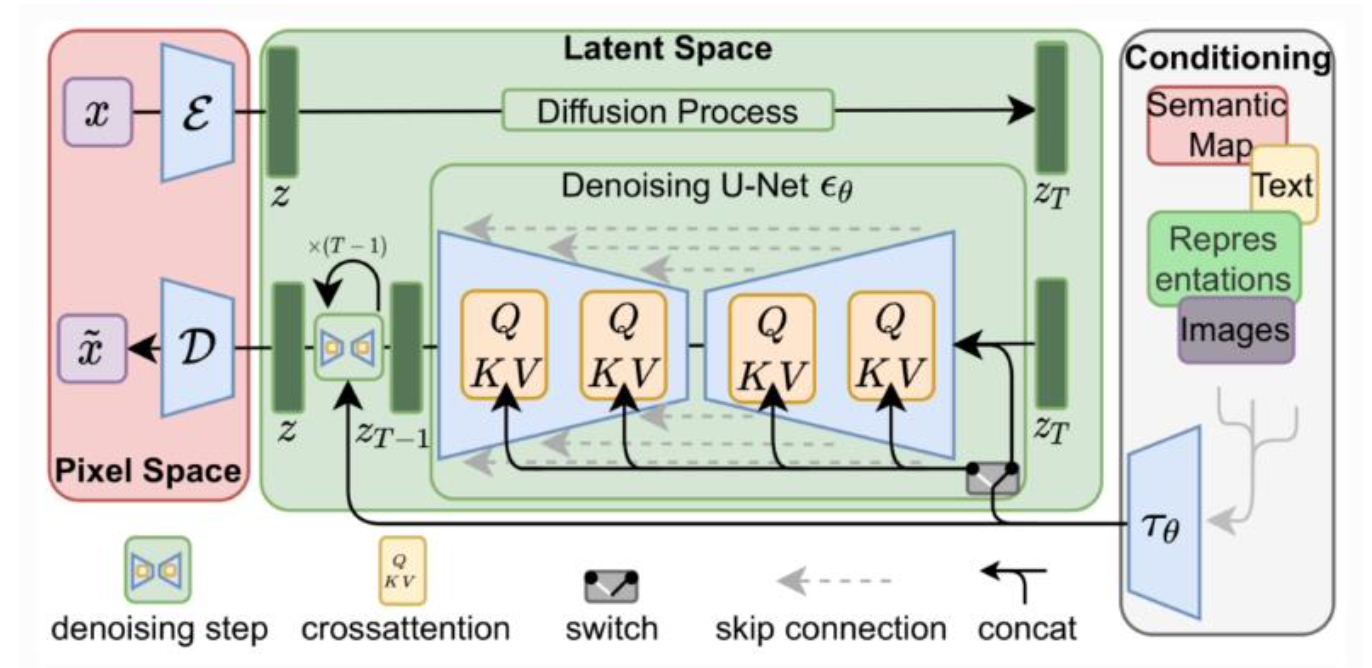
\includegraphics[width=0.6\textwidth]{figure/StableDiffusionArchitecture.png}
    \caption{Architettura completa della Stable Diffusion.}
    \label{fig:StabDiffArch}
\end{figure}

\subsubsection{Cross-Attention nel Perceiver IO}

Il \textbf{Perceiver IO} è un'architettura multimodale in grado di gestire input e output eterogenei. Utilizza la Cross-Attention per mescolare input multimodali in una rappresentazione latente compatta, permettendo poi la generazione di output flessibili e controllabili.

\section{Ulteriori forme di Conditioning}
Il testo non è l’unico modo per guidare la generazione. Stable Diffusion e i suoi derivati permettono anche di condizionare il processo su altre informazioni, come bordi, profondità o pose. Queste varianti consentono un controllo più preciso e mirato sull’immagine generata.

\subsection{Image-to-Image}
Nel metodo \textbf{Image-to-Image}, un’immagine di partenza e un prompt testuale vengono utilizzati insieme per produrre una nuova immagine. Questo approccio, introdotto con \textit{SDEdit}, segue questi passaggi:

\begin{enumerate}
    \item L’immagine viene codificata nello spazio latente;
    \item Si aggiunge una quantità controllata di rumore;
    \item La U-Net predice il rumore in base al prompt;
    \item Il rumore stimato viene sottratto e il processo ripetuto più volte;
    \item L’immagine finale viene decodificata tramite il VAE.
\end{enumerate}

\subsection{Depth-to-Image}
Il metodo \textbf{Depth-to-Image} estende il precedente introducendo una mappa di profondità, ottenuta tramite il modello MiDaS. Questa aggiunta fornisce informazioni strutturali sulla scena, migliorando la coerenza spaziale dell’immagine generata.

\begin{enumerate}
    \item Si codifica l’immagine nello spazio latente;
    \item Si estrae la mappa di profondità con MiDaS;
    \item Si aggiunge rumore controllato;
    \item La U-Net predice il rumore condizionata su prompt e profondità;
    \item Si rimuove progressivamente il rumore e si decodifica l’immagine finale.
\end{enumerate}

\section{Classifier Guidance e aggiornamenti della Stable Diffusion}
Nei modelli di diffusione condizionati, un aspetto fondamentale è la capacità di guidare il processo generativo in modo preciso verso un risultato desiderato. A tal fine sono state introdotte due tecniche chiave: il \textbf{Classifier Guidance} e il successivo \textbf{Classifier-Free Guidance} (CFG). Entrambe mirano a controllare il contenuto dell’immagine generata, ma con approcci concettualmente diversi.  

\subsection{Classifier Guidance}
Il \textbf{Classifier Guidance} rappresenta la prima estensione importante dei modelli di diffusione condizionati. L’idea alla base è intuitiva: aggiungere una "forza" esterna che spinga la generazione verso una determinata direzione semantica, come una classe, un oggetto o uno stile desiderato. In altre parole, si vuole che l’immagine non sia solo coerente, ma anche \textit{più fedele} alla condizione imposta (e.g "gatto", "tramonto", "in stile Van Gogh").

\subsubsection{Intuizione di base}
Durante la generazione, il modello di denoising (ad esempio una U-Net) produce a ogni step un’immagine leggermente meno rumorosa. Il Classifier Guidance introduce un secondo modello, un \textbf{classificatore}, che valuta quanto l’immagine corrente corrisponde alla condizione desiderata. La sua derivata rispetto all’immagine latente indica in che direzione modificare il processo di denoising per aumentare la probabilità della condizione voluta. In pratica, questo gradiente funziona come una bussola: il classificatore indica la direzione nel "paesaggio probabilistico" che porta verso immagini più coerenti con la condizione desiderata.

\subsubsection{Formalizzazione Matematica}
Nel caso di una generazione condizionata su una variabile $y$, vogliamo campionare da $p(x_0 | y)$, cioè generare immagini coerenti con la condizione $y$. Possiamo esprimere il gradiente di questa distribuzione come:
\begin{equation}
    \nabla_x \log p(x_t|y) = \nabla_x \log p(x_t) + \nabla_x \log p(y|x_t)
\end{equation}

dove:
\begin{itemize}
    \item $x_t$ è lo stato latente (rumoroso) al tempo $t$;
    \item $p(x_t)$ rappresenta la distribuzione incondizionata appresa dal modello di diffusione;
    \item $p(y|x_t)$ è la probabilità, stimata da un classificatore, che lo stato corrente corrisponda alla condizione desiderata $y$.
\end{itemize}
Il primo termine è ciò che il modello generativo apprende normalmente; il secondo termine, fornito dal classificatore, aggiunge la spinta verso la condizione $y$. Durante la diffusione inversa, questo gradiente viene usato per modificare la previsione del rumore della U-Net:

\begin{equation}
    \epsilon_\theta^{\operatorname{guided}} = \epsilon_\theta(x_t,t) - s \cdot \sigma_t \cdot \nabla_{x_t}\log p(y|x_t)
\end{equation}

dove:
\begin{itemize}
    \item $\epsilon_\theta(x_t,t)$ è il rumore stimato dal modello generativo;
    \item $s$ è un coefficiente che controlla l’intensità della guida;
    \item $\sigma_t$ è la deviazione standard del rumore al passo $t$.
\end{itemize}

Aumentando $s$, il modello viene "spinto" più fortemente verso immagini che il classificatore considera coerenti con la condizione desiderata, ma se $s$ è troppo alto si rischia di perdere diversità o introdurre artefatti visivi.

\subsection{Classifier-Free Guidance (CFG)}
Sebbene efficace, il Classifier Guidance richiede un classificatore esterno, addestrato separatamente. Questo rende l’approccio più complesso e meno flessibile. Per semplificare, nasce il \textbf{Classifier-Free Guidance (CFG)}, oggi utilizzato in modelli come Stable Diffusion, Imagen e DALL-E 3.

\subsubsection{Intuizione}

Nel CFG non si usa un classificatore esplicito. Si addestra invece lo stesso modello generativo a lavorare in due modalità:
\begin{itemize}
    \item \textbf{Condizionata:} quando riceve il prompt testuale $y$;
    \item \textbf{Incondizionata:} quando genera senza prompt (solo dal rumore).
\end{itemize}
Durante la generazione, si combinano le due previsioni per controllare quanto il risultato finale debba aderire al prompt testuale. Formalmente:

\begin{equation}
    \epsilon_\theta^{\operatorname{guided}} = (1 + w)\cdot\epsilon_\theta(x_t,t,y) - w\cdot\epsilon_\theta(x_t,t)
\end{equation}

dove:
\begin{itemize}
    \item $\epsilon_\theta(x_t,t,y)$ è la predizione condizionata (con prompt);
    \item $\epsilon_\theta(x_t,t)$ è quella incondizionata (senza prompt);
    \item $w$ è un iperparametro che regola la forza della guida (\textit{guidance scale}), tipicamente compreso tra 1.5 e 7.5.
\end{itemize}

Quando $w = 0$, il modello ignora completamente il prompt e genera in modo casuale; quando $w$ aumenta, il modello segue più rigidamente le istruzioni testuali, generando immagini più coerenti ma anche meno varie. Questa strategia consente di ottenere un controllo fine sull’aderenza semantica, senza la complessità di un classificatore aggiuntivo. Inoltre, il CFG ha dimostrato empiricamente di fornire risultati visivamente superiori e più coerenti con il testo rispetto al Classifier Guidance tradizionale.

\subsection{Stable Diffusion 2.0 e versioni successive}
Con la diffusione mondiale di Stable Diffusion, sono state introdotte numerose versioni migliorate del modello, ciascuna con affinamenti architetturali e prestazionali. Le principali innovazioni introdotte a partire dalla versione 2.0 includono:

\begin{itemize}
    \item \textbf{Addestramento su risoluzioni più elevate} (es. 768x768), per ottenere immagini nitide e dettagliate;
    \item \textbf{Nuovi text encoder} (e.g OpenCLIP), n grado di comprendere in modo più preciso la semantica dei prompt complessi;
    \item \textbf{Depth-conditioning} nativamente integrato, per generazioni controllate tramite mappe di profondità;
    \item \textbf{Miglioramenti al VAE decoder}, riducendo artefatti e distorsioni cromatiche;
    \item \textbf{Introduzione di ControlNet}, un’estensione che consente un controllo esplicito della struttura dell’immagine (pose, bordi, schizzi, profondità, ecc\ldots).
\end{itemize}

Grazie a questi avanzamenti, Stable Diffusion 2.x è diventato un riferimento industriale e accademico per la generazione di immagini controllata. Il suo equilibrio tra efficienza, qualità visiva e flessibilità ha aperto la strada a un’enorme varietà di applicazioni: dall’arte digitale alla pubblicità, fino alla ricerca scientifica e al design industriale. In sintesi, il passaggio da \textit{Classifier Guidance} a \textit{Classifier-Free Guidance} segna una tappa fondamentale nell’evoluzione dei modelli di diffusione: da un approccio supervisionato e complesso, si è giunti a un metodo più snello, stabile e adattabile, oggi alla base dei modelli generativi più avanzati.

% Preambolo richiesto:
% \usepackage{tikz}
% \usetikzlibrary{arrows.meta,positioning,calc}

\begin{figure}[hbtp]
\centering
\resizebox{0.95\textwidth}{!}{
\begin{tikzpicture}[
    node distance=10mm and 18mm,
    >=Latex,
    box/.style={draw, rounded corners, fill=gray!5, inner sep=6pt, minimum height=7mm, text width=2.8cm, align=center},
    op/.style={draw, rounded corners, fill=blue!6, inner sep=6pt, minimum height=7mm, text width=3.5cm, align=center},
    comb/.style={draw, rounded corners, fill=orange!10, inner sep=6pt, minimum height=7mm, text width=4.5cm, align=center},
    note/.style={font=\footnotesize, align=center},
    title/.style={font=\bfseries, align=center},
    every node/.style={font=\small}
]

% ===================== TOP: CLASSIFIER GUIDANCE =====================
\node[title] (Ttitle) {Classifier Guidance};

\node[box, below=4mm of Ttitle] (xT) {$\mathbf{x}_t$\\(rumore / latente)};
\node[op, right=of xT] (unetT) {U--Net Denoiser\\$\epsilon_\theta(\mathbf{x}_t,t)$};
\node[op, above=of unetT, yshift=5mm] (clf) {Classificatore\\$p(y \mid \mathbf{x}_t)$};
\node[comb, right=of unetT] (guideT) {$\epsilon^{\text{guided}} = \epsilon_\theta - s \, \sigma_t \, \nabla_{\mathbf{x}_t} \log p(y \mid \mathbf{x}_t)$};
\node[box, right=of guideT] (xTm1) {$\mathbf{x}_{t-1}$};

% arrows
\draw[->] (xT) -- (unetT);
\draw[->] (xT) |- (clf.west);
\draw[->] (clf) -| node[pos=0.35, above, note] {$\nabla_{\mathbf{x}_t} \log p(y \mid \mathbf{x}_t)$} (guideT);
\draw[->] (unetT) -- (guideT);
\draw[->] (guideT) -- (xTm1);

% notes
\node[note, below=1mm of unetT] (sigma) {$\sigma_t$: deviazione standard del rumore al passo $t$};
\node[note, below=1mm of guideT] {$s$: intensità della guida};

\draw[dashed, rounded corners] ($(xT.north west)+(-4mm,4mm)$) rectangle ($(xTm1.south east)+(4mm,-10mm)$);

% ===================== BOTTOM: CLASSIFIER-FREE GUIDANCE =====================
\node[title, below=40mm of Ttitle] (Btitle) {Classifier--Free Guidance (CFG)};

\node[box, below=4mm of Btitle] (xB) {$\mathbf{x}_t$\\(rumore / latente)};
\node[op, right=20mm of xB, yshift=12mm] (unetCond) {U--Net condizionata\\$\epsilon_\theta(\mathbf{x}_t,t,y)$};
\node[op, right=20mm of xB, yshift=-10mm] (unetUnc) {U--Net non condizionata\\$\epsilon_\theta(\mathbf{x}_t,t)$};
\node[comb, right=75mm of xB] (mix) {$(1+w)\,\epsilon_\theta(\mathbf{x}_t,t,y) - w\,\epsilon_\theta(\mathbf{x}_t,t)$};
\node[box, right=of mix] (xBm1) {$\mathbf{x}_{t-1}$};

% arrows
\draw[->] (xB) -- ++(18mm,0) |- (unetCond.west);
\draw[->] (xB) -- ++(18mm,0) |- (unetUnc.west);
\draw[->] (unetCond) -| (mix);
\draw[->] (unetUnc) -| (mix);
\draw[->] (mix) -- (xBm1);

\node[note, above=2mm of unetCond] (prompt) {prompt $y$};
\draw[->, shorten >=2pt] (prompt) -- (unetCond);

\node[note, below=1mm of mix] {$w$: guidance scale (aderenza al prompt)};

\draw[dashed, rounded corners] ($(xB.north west)+(-4mm,4mm)$) rectangle ($(xBm1.south east)+(4mm,-10mm)$);

% ===================== LEGEND =====================
\node[note, below=20mm of $(xB)!0.5!(mix)$, text width=11cm] (legend) 
{Legenda: la U--Net stima il rumore; i blocchi arancioni combinano le stime per guidare il passaggio $\mathbf{x}_t \rightarrow \mathbf{x}_{t-1}$. 
Nel \textit{Classifier Guidance} la guida proviene da un classificatore esterno, 
mentre nel \textit{Classifier--Free Guidance} è ottenuta combinando le predizioni condizionata e incondizionata con il fattore $w$.};

\end{tikzpicture}}
\caption{Confronto tra \textbf{Classifier Guidance} (in alto) e \textbf{Classifier--Free Guidance} (in basso). 
Nel primo, la direzione di guida deriva da un classificatore esterno; nel secondo, la guida è interna al modello e regolata dal parametro $w$.}
\label{fig:guidance_vs_cfg}
\end{figure}



\section*{Approfondimenti}

\subsubsection*{DDPM (Denoising Diffusion Probabilistic Models)}

I \textbf{DDPM} rappresentano il framework classico dei modelli di diffusione, introdotti da Ho et al. 2020~\cite{ho2020denoising}. Il processo è modellato come una catena Markoviana di lunghezza $T$, con una forward process che aggiunge rumore gaussianamente e una reverse process approssimata da una rete neurale. Il modello apprende a predire il rumore $\boldsymbol{\epsilon}$ iniettato in $x_t$:
\begin{equation}
    \mathcal{L_{\operatorname{simple}}} = \mathbb{E}_{t,x_{0},\epsilon}[\|\epsilon - \epsilon_\theta(x_t,t)\|^2]
\end{equation}

Pur offrendo alta qualità, il sampling è lento (richiede centinaia di passaggi).

\subsubsection*{DDIM (Denoising Diffusion Implicit Models)}

Proposto da Song et al. (2021)~\cite{song2021score}, \textbf{DDIM} permette un processo di campionamento deterministico (non stocastico), più rapido ed efficiente. Invece di ricampionare il rumore a ogni step, l'algoritmo definisce una traiettoria implicita nell’input space:
\begin{equation}
    x_{t-1} = \sqrt{\alpha_{t-1}}\cdot x_0 + \sqrt{1-\alpha_{t-1}}\cdot\epsilon_t
\end{equation}

DDIM consente di ridurre il numero di step di generazione (e.g da 1000 a 50) senza perdita significativa di qualità.

\subsubsection*{Score-based Generative Models}

Questi modelli, sviluppati in parallelo ai DDPM, si fondano sull’apprendimento dello \textbf{score function} $\nabla_{x} \log p(x_t)$, sfruttando tecniche di Stochastic Differential Equations (SDEs). Le score functions vengono apprese a diversi livelli di rumore, e successivamente usate in una reverse SDE per il sampling. La connessione tra questi modelli e i DDPM è stata formalizzata, rendendoli due facce della stessa medaglia: i DDPM sono una discretizzazione specifica di un processo continuo definito dalle SDE.

\subsection*{ControlNet: Controllo strutturato nella generazione}

\textbf{ControlNet} è un'estensione di Stable Diffusion che consente di aggiungere forti vincoli spaziali o semantici durante la generazione di immagini, preservando fedelmente la struttura in input.

\subsubsection*{Motivazione}

La generazione condizionata solo sul testo può risultare ambigua o imprecisa rispetto a vincoli geometrici desiderati (pose, silhouette, contorni, ecc.). ControlNet introduce un secondo input (es. mappa di pose, bordi Canny, depth map), utilizzato per controllare la generazione a livello strutturale.

\subsubsection*{Architettura}

ControlNet replica la U-Net di Stable Diffusion, inizializzandola con i pesi pre-addestrati, ma aggiunge dei \textbf{moduli di controllo} (ad es. convolutioni residue) che elaborano l’input strutturale. Questi moduli sono inizialmente disattivati (zero-conv) e vengono addestrati separatamente. Durante il training, il modello apprende come combinare la guida testuale (prompt) e quella strutturale, garantendo coerenza visiva e semantica.

\subsubsection*{Tipologie di controllo supportate}

ControlNet supporta diverse modalità di conditioning:

\begin{itemize}
    \item \textbf{Pose estimation (OpenPose):} genera persone in pose specifiche;
    \item \textbf{Canny edges:} preserva bordi di oggetti o silhouette;
    \item \textbf{Scribble / Sketch:} permette agli utenti di disegnare forme rudimentali;
    \item \textbf{Depth maps:} rispetta la disposizione spaziale degli oggetti;
    \item \textbf{Normal maps:} per superfici e orientamenti 3D.
\end{itemize}

Questa flessibilità rende ControlNet uno strumento potente per applicazioni artistiche, design, fashion, architettura e prototipazione visiva.

\subsection*{Modelli a confronto}

\begin{sidewaystable}[htbp]
    \centering
    \caption{Confronto tra principali modelli di generazione di immagini}
    \begin{tabularx}{\textwidth}{|l|X|X|X|X|}
    \hline
    \textbf{Caratteristica} & \textbf{Stable Diffusion} & \textbf{DALL·E 2} & \textbf{Midjourney} & \textbf{Imagen} \\
    \hline
    \textbf{Architettura} & Diffusione latente (VAE + U-Net + CLIP) & Diffusione con VQGAN e CLIP & Proprietaria (non pubblicata) & Diffusione pura + T5 encoder \\
    \hline
    \textbf{Accessibilità} & Open source, estendibile & Accesso tramite API OpenAI & Solo via Discord (chiuso) & Non disponibile al pubblico \\
    \hline
    \textbf{Controllabilità} & Alta: ControlNet, CFG, img2img & Limitata & Bassa, prompt tuning empirico & Alta, ma solo testata internamente \\
    \hline
    \textbf{Qualità visiva} & Molto alta (variabile con CFG) & Alta, dettagli precisi & Alta, stile molto curato & Eccellente, fotorealistico \\
    \hline
    \textbf{Customizzazione} & Altissima (plugin, estensioni, modelli LoRA) & Limitata & Nessuna & Nessuna \\
    \hline
    \textbf{Prompt understanding} & Buono (dipende dal modello CLIP) & Ottimo & Medio-alto & Eccellente (T5 encoder) \\
    \hline
    \textbf{Uso offline} & Sì (tutto in locale) & No & No & No \\
    \hline
\end{tabularx}
\end{sidewaystable}


\begin{Osservazione}
    \textbf{Stable Diffusion} è la soluzione preferita per chi desidera pieno controllo, estensibilità e utilizzo locale. Supporta l’intero ecosistema open-source, inclusi modelli LoRA, ControlNet, DreamBooth, ecc.
\end{Osservazione}
\begin{Osservazione}
    \textbf{DALL-E 2} è adatto a chi cerca semplicità d’uso e buone prestazioni, ma con meno flessibilità.
\end{Osservazione}
\begin{Osservazione}
    \textbf{Midjourney} produce risultati artisticamente curati e stilizzati, ma non offre controllo diretto sulla struttura.
\end{Osservazione}
\begin{Osservazione}
    \textbf{Imagen}, pur dimostrando risultati eccezionali nei paper, non è accessibile pubblicamente per motivi di sicurezza e bias.
\end{Osservazione}

\subsection*{Prompt Engineering}

Prompt ben progettati sono essenziali per ottenere immagini coerenti e di qualità. Un prompt efficace include:

\begin{itemize}
    \item \textbf{Soggetto primario:} "a futuristic city skyline";
    \item \textbf{Modificatori visivi:} "at night, with neon lights";
    \item \textbf{Stile:} "cyberpunk, digital art, trending on ArtStation";
    \item \textbf{Fotografia:} "wide-angle, bokeh, depth of field";
    \item \textbf{Compositing:} "symmetrical composition, ultra-detailed".
\end{itemize}

\subsubsection*{Prompt negativo}

Stable Diffusion supporta anche \textbf{prompt negativi}, usati per escludere elementi indesiderati:

\begin{quote}[scale=0.9]
    \texttt{--negative\_prompt="blurry, low resolution, bad anatomy, extra limbs, disfigured"}
\end{quote}

Questi aiutano a ridurre artefatti e risultati indesiderati.

\subsubsection*{Prompt chaining e combinazioni}

Tecniche avanzate includono:
\begin{itemize}
    \item \textbf{Prompt chaining:} usare l’immagine generata da un prompt come base per il successivo (img2img);
    \item \textbf{Attention weighting:} parentesi per controllare l'importanza di certe parole: \texttt{(cat:1.3)}, \texttt{[tree:0.5]};
    \item \textbf{Multiple subjects:} separati da "AND" o virgole per composizioni complesse.
\end{itemize}

\subsubsection*{Token embedding personalizzati}

È possibile introdurre token personalizzati (es. \texttt{<sks style>}, \texttt{<johndoe face>}) associati a concetti specifici via fine-tuning o DreamBooth, utili in contesti professionali (moda, branding, VFX).